% MATLAB source: paper/plot_existing_manuscript_figures.m
\begin{figure}[tbp]
  \centering
  \begin{subfigure}[t]{0.94\linewidth}
    \centering
    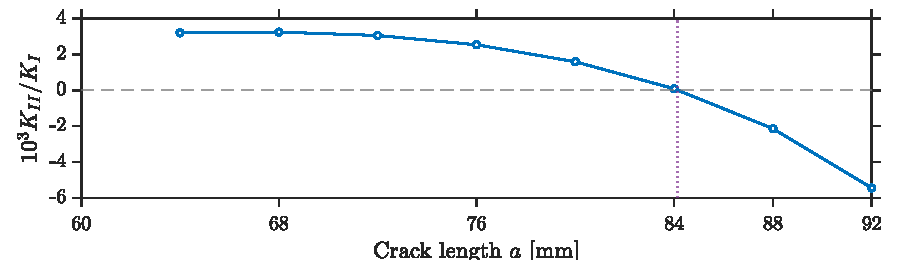
\includegraphics[width=\linewidth]{figures/late/mode_mixity.pdf}
    \caption{Late mode-mixity history.}
    \label{fig:late-mixity}
  \end{subfigure}

  \medskip

  \begin{subfigure}[t]{0.94\linewidth}
    \centering
    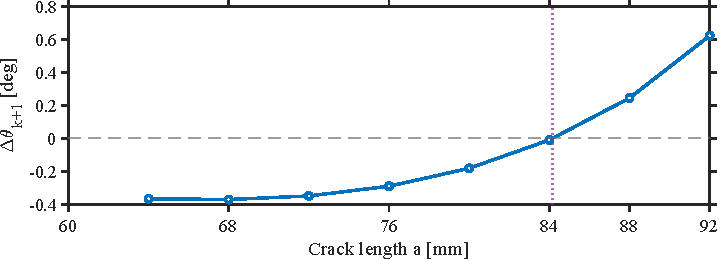
\includegraphics[width=\linewidth]{figures/late/turn.pdf}
    \caption{Incremental MTS turn relative to the current segment.}
    \label{fig:late-turn}
  \end{subfigure}

  \caption{Mode-mixity sign reversal and opposite-signed MTS turning.
  Each marker is an accepted current-tip state; its turn predicts the next
  segment. The vertical dotted line is the interpolated $K_{II}/K_I=0$
  location. The positive turn reported at $a=92$ mm belongs to the $P_{23}$
  solution and predicts the unsolved next geometry.}
  \label{fig:late}
\end{figure}
